\subsection{Задача 1}

\subsubsection{а)}
\begin{tikzpicture}[level/.style={sibling distance=60mm/#1}, scale=0.6]
\node [cir] {$ \lor $}
  child { 
    node [cir] {$ \land $} 
    child {node [cir] {A}} 
    child {node [cir] {B}}
    edge from parent node[above left] {$ \lnot $}
  }
  child { 
    node [cir] {$ \land $}
    child {node [cir] {A}}
    child {node [cir] {B}}
  };
\end{tikzpicture}

\rule{0cm}{0cm}

\begin{tabular}{|c|c|c|}
  \hline
  A & B & $ \lnot (A \land B) \lor (A \land B) $ \\\hline
  0 & 0 & 1 \\\hline
  0 & 1 & 1 \\\hline
  1 & 0 & 1 \\\hline
  1 & 1 & 1 \\\hline
\end{tabular}


\subsubsection{б)}
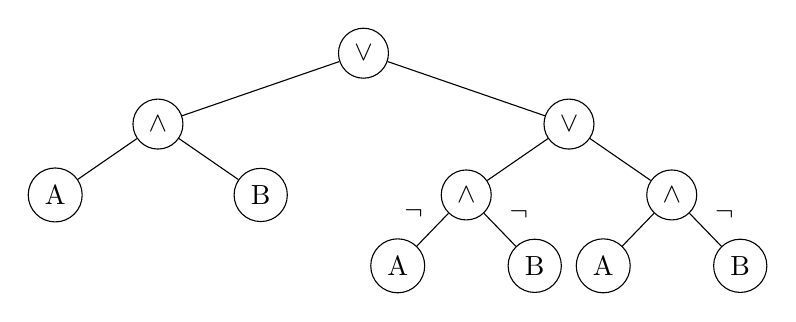
\begin{tikzpicture}[level/.style={sibling distance=87mm/#1}, scale=0.6]
\node [circle, draw=black] {$ \lor $}
  child { 
    node [circle, draw=black] {$ \land $}
    child { node [circle, draw=black] {A} }
    child { node [circle, draw=black] {B} }
  }
  child {
    node [circle, draw=black] {$ \lor $}
    child { 
      node [circle, draw=black] {$ \land $} 
      child { 
        node [circle, draw=black] {A} 
        edge from parent node[above left] {$ \lnot $}
      }
      child { 
        node [circle, draw=black] {B} 
        edge from parent node[above right] {$ \lnot $}
      }
    }
    child { 
      node [circle, draw=black] {$ \land $} 
      child { node [circle, draw=black] {A} }
      child { 
        node [circle, draw=black] {B} 
        edge from parent node[above right] {$ \lnot $}
      }
    }
  };
\end{tikzpicture}

\rule{0cm}{0cm}

\begin{tabular}{|c|c|c|}
  \hline
  A & B & $ A \land B \lor \lnot A \land \lnot B \lor A \land \lnot B $ \\\hline
  0 & 0 & 1 \\\hline
  0 & 1 & 0 \\\hline
  1 & 0 & 1 \\\hline
  1 & 1 & 1 \\\hline
\end{tabular}


\subsubsection{в)}
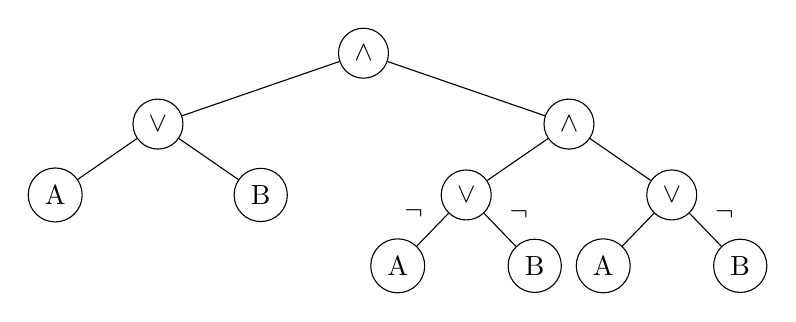
\begin{tikzpicture}[level/.style={sibling distance=87mm/#1}, scale=0.6]
\node [circle, draw=black] {$ \land  $}
  child { 
    node [circle, draw=black] {$ \lor  $}
    child {
      node [circle, draw=black] {A}
    }
    child {
      node [circle, draw=black] {B}
    }
  }
  child {
    node [circle, draw=black] {$ \land  $} child {
      node [circle, draw=black] {$ \lor  $}
      child {
        node [circle, draw=black] {A}
        edge from parent node[above left] {$ \lnot  $}
      }
      child {
        node [circle, draw=black] {B}
        edge from parent node[above right] {$ \lnot  $}
      }
    }
    child {
      node [circle, draw=black] {$ \lor  $}
      child {
        node [circle, draw=black] {A}
      }
      child {
        node [circle, draw=black] {B}
        edge from parent node[above right] {$ \lnot  $}
      }
    }
  };
\end{tikzpicture}

\rule{0cm}{0cm}

\begin{tabular}{|c|c|c|}
  \hline
  A & B & $ (A \lor B) \land (\lnot A \lor \lnot B) \land (A \lor \lnot B) $ \\\hline
  0 & 0 & 0 \\\hline
  0 & 1 & 0 \\\hline
  1 & 0 & 1 \\\hline
  1 & 1 & 0 \\\hline
\end{tabular}


\subsubsection{г)}
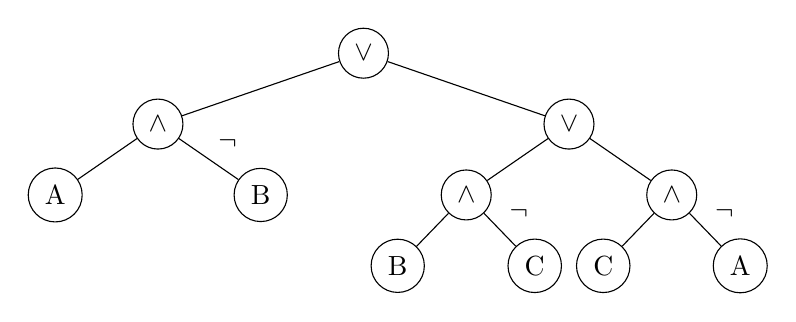
\begin{tikzpicture}[level/.style={sibling distance=87mm/#1}, scale=0.6]
\node [circle, draw=black] {$ \lor  $}
  child { 
    node [circle, draw=black] {$ \land  $}
    child {
      node [circle, draw=black] {A}
    }
    child {
      node [circle, draw=black] {B}
      edge from parent node[above right] {$ \lnot  $}
    }
  }
  child {
    node [circle, draw=black] {$ \lor  $}
    child {
      node [circle, draw=black] {$ \land $}
      child {
        node [circle, draw=black] {B}
      }
      child {
        node [circle, draw=black] {C}
        edge from parent node[above right] {$ \lnot  $}
      }
    }
    child {
      node [circle, draw=black] {$ \land  $}
      child {
        node [circle, draw=black] {C}
      }
      child {
        node [circle, draw=black] {A}
        edge from parent node[above right] {$ \lnot  $}
      }
    }
  };
\end{tikzpicture}

\begin{tabular}{|c|c|c|c|}
  \hline
  A & B & C & $ A \land \lnot B \lor B \land \lnot C \lor C \land \lnot A $ \\\hline
  0 & 0 & 0 & 0 \\\hline
  0 & 0 & 1 & 1 \\\hline
  0 & 1 & 0 & 1 \\\hline
  0 & 1 & 1 & 1 \\\hline
  1 & 0 & 0 & 1 \\\hline
  1 & 0 & 1 & 1 \\\hline
  1 & 1 & 0 & 1 \\\hline
  1 & 1 & 1 & 0 \\\hline
\end{tabular}


\subsubsection{д)}
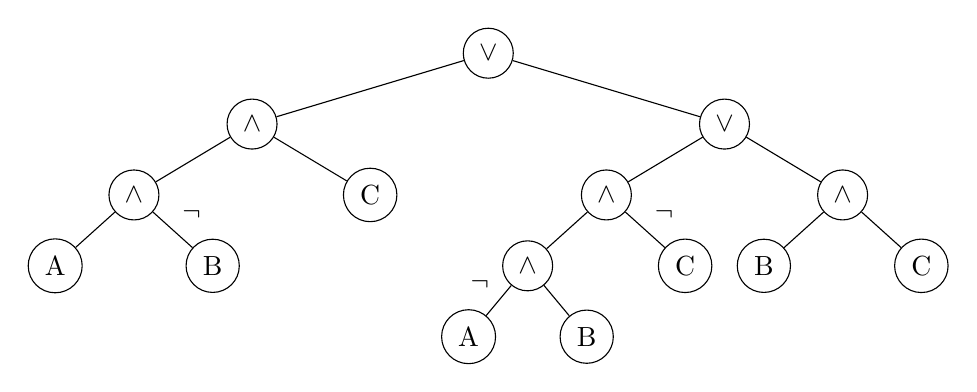
\begin{tikzpicture}[level/.style={sibling distance=100mm/#1}, scale=0.6]
\node [circle, draw=black] {$ \lor  $}
  child { 
    node [circle, draw=black] {$ \land  $}
    child {
      node [circle, draw=black] {$ \land  $}
      child {
        node [circle, draw=black] {A}
      }
      child {
        node [circle, draw=black] {B}
        edge from parent node[above right] {$ \lnot  $}
      }
    }
    child {
      node [circle, draw=black] {C}
    }
  }
  child {
    node [circle, draw=black] {$ \lor  $}
    child {
      node [circle, draw=black] {$ \land  $}
      child {
        node [circle, draw=black] {$ \land  $}
        child {
          node [circle, draw=black] {A}
          edge from parent node[above left] {$ \lnot  $}
        }
        child {
          node [circle, draw=black] {B}
        }
      }
      child {
        node [circle, draw=black] {C}
        edge from parent node[above right] {$ \lnot  $}
      }
    }
    child {
      node [circle, draw=black] {$ \land  $}
      child {
        node [circle, draw=black] {B}
      }
      child {
        node [circle, draw=black] {C}
      }
    }
  };
\end{tikzpicture}

\rule{0cm}{0cm}

\begin{tabular}{|c|c|c|c|}
  \hline
  A & B & C & $ A \land \lnot B \land C \lor \lnot A \land B \land \lnot C \lor B \land C $ \\\hline
  0 & 0 & 0 & 0 \\\hline
  0 & 0 & 1 & 0 \\\hline
  0 & 1 & 0 & 1 \\\hline
  0 & 1 & 1 & 1 \\\hline
  1 & 0 & 0 & 0 \\\hline
  1 & 0 & 1 & 1 \\\hline
  1 & 1 & 0 & 0 \\\hline
  1 & 1 & 1 & 1 \\\hline
\end{tabular}


\subsubsection{е)}
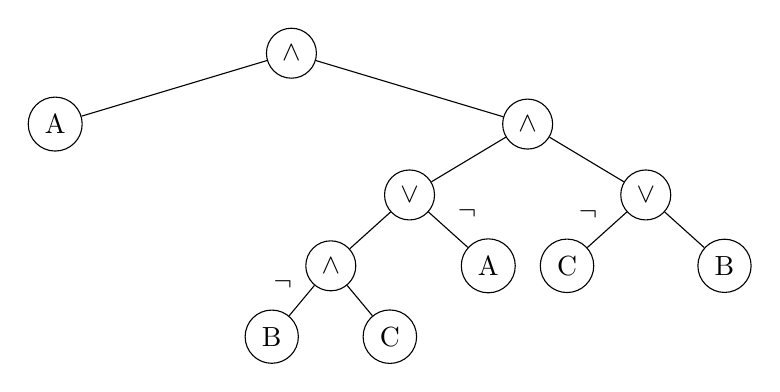
\begin{tikzpicture}[level/.style={sibling distance=100mm/#1}, scale=0.6]
\node [circle, draw=black] {$ \land  $}
  child { 
    node [circle, draw=black] {A}
  }
  child {
    node [circle, draw=black] {$ \land  $}
    child {
      node [circle, draw=black] {$ \lor  $}
      child {
        node [circle, draw=black] {$ \land  $}
        child {
          node [circle, draw=black] {B}
          edge from parent node[above left] {$ \lnot  $}
        }
        child {
          node [circle, draw=black] {C}
        }
      }
      child {
        node [circle, draw=black] {A}
        edge from parent node[above right] {$ \lnot  $}
      }
    }
    child {
      node [circle, draw=black] {$ \lor  $}
      child {
        node [circle, draw=black] {C}
        edge from parent node[above left] {$ \lnot  $}
      }
      child {
        node [circle, draw=black] {B}
      }
    }
  };
\end{tikzpicture}

\rule{0cm}{0cm}

\begin{tabular}{|c|c|c|c|}
  \hline
  A & B & C & $ A \land (\lnot B \land C \lor \lnot A) \land (\lnot C \lor B) $ \\\hline
  0 & 0 & 0 & 0 \\\hline
  0 & 0 & 1 & 0 \\\hline
  0 & 1 & 0 & 0 \\\hline
  0 & 1 & 1 & 0 \\\hline
  1 & 0 & 0 & 0 \\\hline
  1 & 0 & 1 & 0 \\\hline
  1 & 1 & 0 & 0 \\\hline
  1 & 1 & 1 & 0 \\\hline
\end{tabular}


\subsubsection{ж)}
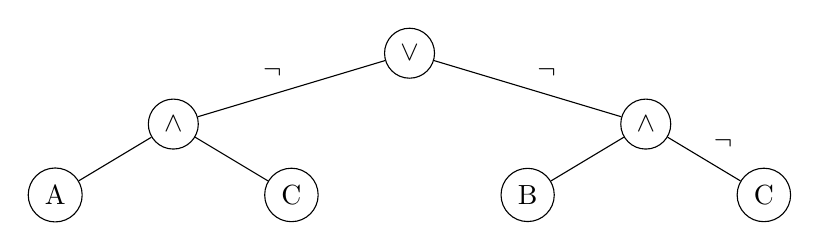
\begin{tikzpicture}[level/.style={sibling distance=100mm/#1}, scale=0.6]
\node [circle, draw=black] {$ \lor  $}
  child { 
    node [circle, draw=black] {$ \land  $}
    child {
      node [circle, draw=black] {A}
    }
    child {
      node [circle, draw=black] {C}
    }
    edge from parent node[above left] {$ \lnot  $}
  }
  child {
    node [circle, draw=black] {$ \land  $}
    child {
      node [circle, draw=black] {B}
    }
    child {
      node [circle, draw=black] {C}
      edge from parent node[above right] {$ \lnot  $}
    }
    edge from parent node[above right] {$ \lnot  $}
  };
\end{tikzpicture}

\rule{0cm}{0cm}

\begin{tabular}{|c|c|c|c|}
  \hline
  A & B & C & $ \lnot (A \land B) \lor \lnot (B \land \lnot C) $ \\\hline
  0 & 0 & 0 & 1 \\\hline
  0 & 0 & 1 & 1 \\\hline
  0 & 1 & 0 & 1 \\\hline
  0 & 1 & 1 & 1 \\\hline
  1 & 0 & 0 & 1 \\\hline
  1 & 0 & 1 & 1 \\\hline
  1 & 1 & 0 & 0 \\\hline
  1 & 1 & 1 & 1 \\\hline
\end{tabular}

\subsubsection{з)}
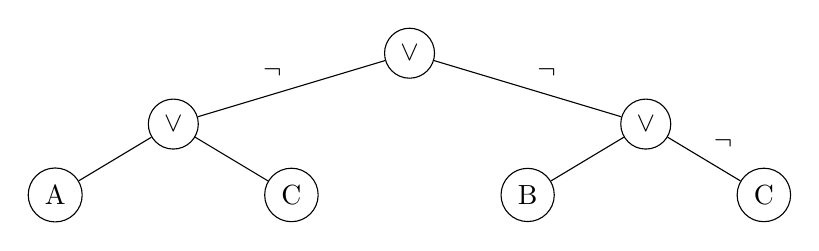
\begin{tikzpicture}[level/.style={sibling distance=100mm/#1}, scale=0.6]
\node [circle, draw=black] {$ \lor  $}
  child { 
    node [circle, draw=black] {$ \lor  $}
    child {
      node [circle, draw=black] {A}
    }
    child {
      node [circle, draw=black] {C}
    }
    edge from parent node[above left] {$ \lnot  $}
  }
  child {
    node [circle, draw=black] {$ \lor  $}
    child {
      node [circle, draw=black] {B}
    }
    child {
      node [circle, draw=black] {C}
      edge from parent node[above right] {$ \lnot  $}
    }
    edge from parent node[above right] {$ \lnot  $}
  };
\end{tikzpicture}

\rule{0cm}{0cm}

\begin{tabular}{|c|c|c|c|}
  \hline
  A & B & C & $ \lnot (A \lor B) \lor \lnot (B \lor \lnot C) $ \\\hline
  0 & 0 & 0 & 1 \\\hline
  0 & 0 & 1 & 1 \\\hline
  0 & 1 & 0 & 0 \\\hline
  0 & 1 & 1 & 0 \\\hline
  1 & 0 & 0 & 0 \\\hline
  1 & 0 & 1 & 1 \\\hline
  1 & 1 & 0 & 0 \\\hline
  1 & 1 & 1 & 0 \\\hline
\end{tabular}


\subsubsection{и)}

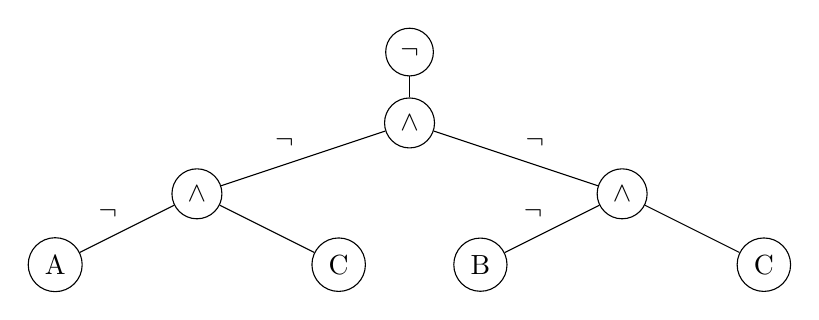
\begin{tikzpicture}[level/.style={sibling distance=180mm/#1}, scale=0.6]
\node [circle, draw=black] {$ \lnot  $}
  child { 
    node [circle, draw=black] {$ \land  $}
    child { 
      node [circle, draw=black] {$ \land  $}
      child {
        node [circle, draw=black] {A}
        edge from parent node[above left] {$ \lnot  $}
      }
      child {
        node [circle, draw=black] {C}
      }
      edge from parent node[above left] {$ \lnot  $}
    }
    child { 
      node [circle, draw=black] {$ \land  $}
      child {
        node [circle, draw=black] {B}
        edge from parent node[above left] {$ \lnot  $}
      }
      child {
        node [circle, draw=black] {C}
      }
      edge from parent node[above right] {$ \lnot  $}
    }
  };
\end{tikzpicture}

\rule{0cm}{0cm}

\begin{tabular}{|c|c|c|c|}
  \hline
  A & B & C & $ \lnot (\lnot (\lnot A \land C) \land \lnot (\lnot B \land C)) $ \\\hline
  0 & 0 & 0 & 0 \\\hline
  0 & 0 & 1 & 1 \\\hline
  0 & 1 & 0 & 0 \\\hline
  0 & 1 & 1 & 1 \\\hline
  1 & 0 & 0 & 0 \\\hline
  1 & 0 & 1 & 1 \\\hline
  1 & 1 & 0 & 0 \\\hline
  1 & 1 & 1 & 0 \\\hline
\end{tabular}

\subsubsection{к)}
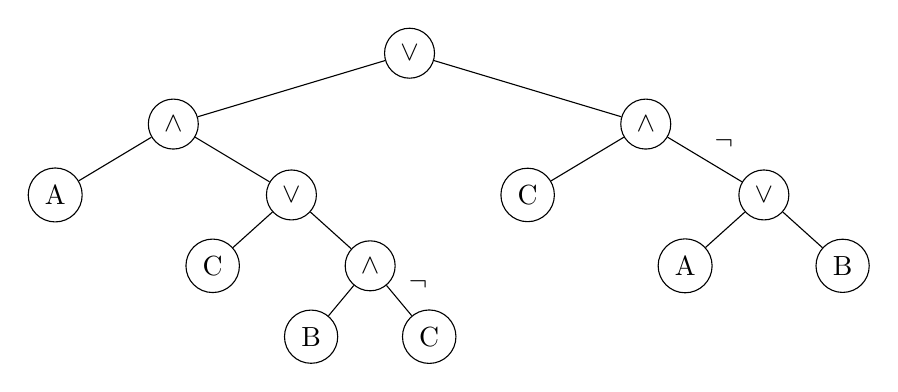
\begin{tikzpicture}[level/.style={sibling distance=100mm/#1}, scale=0.6]
\node [circle, draw=black] {$ \lor  $}
  child { 
    node [circle, draw=black] {$ \land  $}
    child {
      node [circle, draw=black] {A}
    }
    child {
      node [circle, draw=black] {$ \lor $}
      child {
        node [circle, draw=black] {C}
      }
      child {
        node [circle, draw=black] {$ \land  $}
        child {
          node [circle, draw=black] {B}
        }
        child {
          node [circle, draw=black] {C}
          edge from parent node[above right] {$ \lnot  $}
        }
      }
    }
  }
  child {
    node [circle, draw=black] {$ \land  $}
    child {
      node [circle, draw=black] {C}
    }
    child {
      node [circle, draw=black] {$ \lor  $}
      child {
        node [circle, draw=black] {A}
      }
      child {
        node [circle, draw=black] {B}
      }
      edge from parent node[above right] {$ \lnot  $}
    }
  };
\end{tikzpicture}

\rule{0cm}{0cm}

\begin{tabular}{|c|c|c|c|}
  \hline
  A & B & C & $ A \land (C \lor B \land \lnot C) \lor C \land \lnot (A \lor B) $ \\\hline
  0 & 0 & 0 & 0 \\\hline
  0 & 0 & 1 & 1 \\\hline
  0 & 1 & 0 & 0 \\\hline
  0 & 1 & 1 & 0 \\\hline
  1 & 0 & 0 & 0 \\\hline
  1 & 0 & 1 & 1 \\\hline
  1 & 1 & 0 & 1 \\\hline
  1 & 1 & 1 & 1 \\\hline
\end{tabular}


\subsubsection{л)}
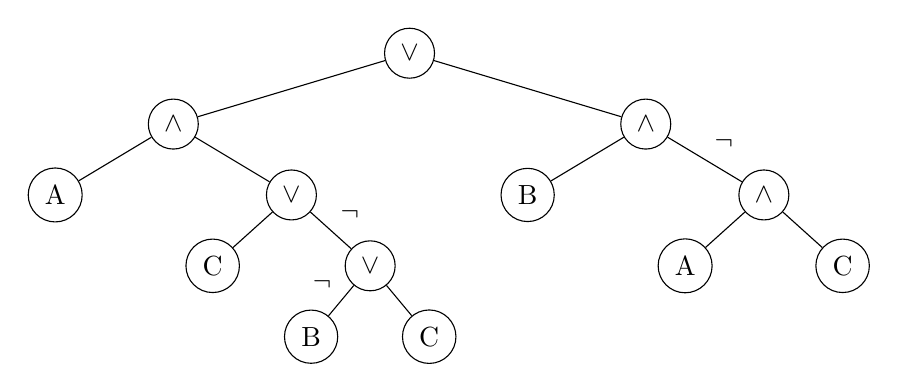
\begin{tikzpicture}[level/.style={sibling distance=100mm/#1}, scale=0.6]
\node [circle, draw=black] {$ \lor  $}
  child { 
    node [circle, draw=black] {$ \land  $}
    child {
      node [circle, draw=black] {A}
    }
    child {
      node [circle, draw=black] {$ \lor  $}
      child {
        node [circle, draw=black] {C}
      }
      child {
        node [circle, draw=black] {$ \lor  $}
        child {
          node [circle, draw=black] {B}
          edge from parent node[above left] {$ \lnot  $}
        }
        child {
          node [circle, draw=black] {C}
        }
        edge from parent node[above right] {$ \lnot  $}
      }
    }
  }
  child {
    node [circle, draw=black] {$ \land  $}
    child {
      node [circle, draw=black] {B}
    }
    child {
      node [circle, draw=black] {$ \land  $}
      child {
        node [circle, draw=black] {A}
      }
      child {
        node [circle, draw=black] {C}
      }
      edge from parent node[above right] {$ \lnot  $}
    }
  };
\end{tikzpicture}

\rule{0cm}{0cm}

\begin{tabular}{|c|c|c|c|}
  \hline
  A & B & C & $ A \land (C \lor \lnot (\lnot B \lor C)) \lor B \land \lnot (A \land C) $ \\\hline
  0 & 0 & 0 & 0 \\\hline
  0 & 0 & 1 & 0 \\\hline
  0 & 1 & 0 & 1 \\\hline
  0 & 1 & 1 & 1 \\\hline
  1 & 0 & 0 & 0 \\\hline
  1 & 0 & 1 & 1 \\\hline
  1 & 1 & 0 & 1 \\\hline
  1 & 1 & 1 & 1 \\\hline
\end{tabular}
